\documentclass[12pt, aspectratio=43]{beamer}
\usepackage[backend=bibtex, style=authoryear]{biblatex} % bibliography
\usepackage{multirow}
\usepackage{adjustbox}
\usepackage{tikz}
\usepackage{multirow}

% HACKS A CUSTOM COMMANDS
\newcommand{\backupbegin}{
   \newcounter{framenumberappendix}
   \setcounter{framenumberappendix}{\value{framenumber}}
}
\newcommand{\backupend}{
   \addtocounter{framenumberappendix}{-\value{framenumber}}
   \addtocounter{framenumber}{\value{framenumberappendix}} 
}
\def\checkmark{\tikz\fill[scale=0.4](0,.35) -- (.25,0) -- (1,.7) -- (.25,.15) -- cycle;} 

% BEAMER TEMPLATE AND THEME
\setbeamertemplate{footline}[frame number]
\usetheme{Estonia}
\mode<presentation>
\AtBeginSection[]{
  \begin{frame}
  \vfill
  \centering
  \begin{beamercolorbox}[sep=8pt,center,shadow=true,rounded=true]{title}
    \usebeamerfont{title}\insertsectionhead\par%
  \end{beamercolorbox}
  \vfill
  \end{frame}
}

\addbibresource{../biblio.bib}

% TITLE PAGE
\title{Kubernetes cluster simulator based on Batsim}
\title{Development and evaluation of a Kubernetes cluster simulator based on
Batsim}

\author{\textbf{Presented by:} Théo Larue\\\textbf{Supervised by:} Olivier
Richard \& Michael Mercier}

\date{August 31, 2020}

\institute[Théo LARUE]{Université Grenoble Alpes}

\titlegraphic{
	\includegraphics[height=5ex]{../imgs/uga-logo.png}\hspace{2ex}
	\includegraphics[height=6ex]{../imgs/ENSIMAG.png}\hspace{2ex}
	\includegraphics[height=5ex]{../imgs/Logo-LIG.jpg}\hspace{2ex}
	\includegraphics[height=5ex]{../imgs/ryax-logo.png}
}

\begin{document}

\frame{\titlepage}

\begin{frame}{Table of contents}
	\tableofcontents
\end{frame}

\section{Introduction}

\begin{frame}{Resource and Jobs Management System}
	\begin{columns}
		\column{0.7\textwidth}
		The RJMS is at the core of the cluster.
		\begin{exampleblock}{Examples of RJMS}
			\begin{itemize}
				\item OAR
				\item SLURM
				\item HadoopYARN
				\item Apache Mesos
			\end{itemize}
		\end{exampleblock}

		\column{0.3\textwidth}
		\centering
		\includegraphics[scale=0.6]{../imgs/RJMS.pdf}
	\end{columns}
\end{frame}


\begin{frame}{Kubernetes}
	\begin{columns}
		\column{0.7\textwidth}
		\textbf{Kubernetes in a nutshell}
		\begin{itemize}
			\item Open source resource manager for containerized applications
			\item About 2M lines of code
			\item 2.8k contributors
		\end{itemize}

		\column{0.3\textwidth}
		\centering
		\includegraphics[width=\textwidth]{../imgs/kube-logo.png}
	\end{columns}

	\centering
	\includegraphics[width=\textwidth]{../imgs/container_evolution.png}
	\tiny{source: \url{https://kubernetes.io/docs/}}
\end{frame}

\begin{frame}{A component of the RJMS: the scheduler}
	\begin{columns}
		\column{0.5\textwidth}
		\includegraphics[width=\textwidth]{../imgs/gantt_small.png}
		\textbf{Scheduling} is the act of allocating tasks to resources.

		\column{0.5\textwidth}
		\begin{block}{Numerous factors}
			\begin{itemize}
				\item Workloads
				\item Applications
				\item System size
				\item Network topology
				\item Energy consumption
				\item Scheduling policies
			\end{itemize}
		\end{block}

		Complex implementations: Kubernetes default
		scheduler weighs \textbf{47k lines of code}.
	\end{columns}
\end{frame}

\begin{frame}{Studying RJMS}
	\begin{columns}
		\column{0.4\textwidth}
		\textbf{Different approaches}
		\begin{itemize}
			\item Analytical study
			\item Real experiments
			\item Emulation
			\item \textbf{Simulation}
		\end{itemize}

		\column{0.6\textwidth}
		\centering
		\includegraphics[scale=0.3]{../imgs/batsim-logo.png}
		\includegraphics[scale=0.3]{../imgs/simgrid-logo.png}

		\vspace{4ex}

		\includegraphics[scale=0.3]{../imgs/batsim-sequence-diag.png}

		\small{Batsim, an infrastructure simulator aimed at studying RJMS.}
	\end{columns}
\end{frame}

\begin{frame}{Contribution: Batkube}
	\begin{columns}
		\column{0.7\textwidth}
		\includegraphics[width=\textwidth]{../imgs/problematic.pdf}

		\vspace{1cm}

		\includegraphics[width=\textwidth]{../imgs/contribution.pdf}

		\column{0.38\textwidth}
		\begin{exampleblock}{Batkube supports}
			\begin{itemize}
				\item Any Go scheduler
				\item Any cluster size
				\item Resource requests
				\item Non parallel tasks
			\end{itemize}
		\end{exampleblock}
	\end{columns}
\end{frame}

\section{Literature review}

\begin{frame}{Infrastructure simulators}
	\begin{columns}
		\column{0.5\textwidth}
		\begin{adjustbox}{width=\linewidth}
			\begin{tabular}{lccccc}
				\hline
				& \rotatebox[origin=c]{90}{Grid} & \rotatebox[origin=c]{90}{HPC} & \rotatebox[origin=c]{90}{Cloud} & \rotatebox[origin=c]{90}{P2P} & \rotatebox[origin=c]{90}{Volunteer}\\
				\hline
				\hline
				\textbf{SimGrid} & \checkmark & & & &\\
				GridSim & \checkmark & & & &\\
				\hline
				LogGOPSim & & \checkmark & & &\\
				BigSim & & \checkmark & & &\\
				\hline
				CloudSim & & & \checkmark  & &\\
				GroudSim & \checkmark & & \checkmark & &\\
				\hline
				PeerSim & & & & \checkmark &\\
				OverSim & & & & \checkmark &\\
				\hline
				SimBA & & & & & \checkmark \\
				SimBOINC & & & & & \checkmark \\
				\hline
			\end{tabular}
		\end{adjustbox}
		\centering
		{\small Domain specific simulators}

		\column{0.5\textwidth}
		\centering
		\includegraphics[scale=0.3]{../imgs/simgrid-logo.png}\\
		\raggedright
		\textbf{SimGrid}
		\begin{itemize}
			\item Framework for building simulators
			\item Versatile, accurate and scalable
			\item 20 years of experience
			\item Simple analytical models
		\end{itemize}
	\end{columns}
\end{frame}

%\begin{block}{Publication specific simulators}
%\end{block}

\begin{frame}{Simulators for the study of RJMS}
	\begin{columns}
		\column{0.5\textwidth}
		\begin{block}{Often \textit{ad hoc} simulators}
			``Publish and perish'' - Milian Poquet
		\end{block}

		\column{0.5\textwidth}
		\begin{exampleblock}{Some active projects}
			\begin{itemize}
				\item YARNSim
				\item SLURM simulator
			\end{itemize}
		\end{exampleblock}
	\end{columns}

	\vspace{2ex}
	\begin{tabular}{lccc}
		\hline
		& \textbf{Scheduler} & \textbf{Platform} & \textbf{Job model}\\
		\hline\hline
		\textbf{Accasim} & Internal & Ad hoc & Static duration\\
		\textbf{Alea} & Internal & GridSim & Static duration\\
		\textbf{Batsim} & Custom Protocol & SimGrid & SimGrid models\\
		\hline
	\end{tabular}
	\vspace{1ex}
	\centering
	{\small Simulation of RJMS}

\end{frame}

%\begin{frame}{SimGrid}
%	SimGrid: Versatile, scalable, accurate.
%
%	Cpu = a computation speed.\\
%	Storage = a seek time and a data transfert rate.\\
%	Network = a flow model, modeling bandwith sharing behaviors.
%
%	Simple models but thoroughly validated.
%\end{frame}

\begin{frame}{Kubernetes cluster simulation}
	\centering
	\textbf{Kubernetes simulation projects}
	\begin{adjustbox}{width=0.8\textwidth}
		\begin{tabular}{lll}
			\hline
			& \textbf{joySim} & \textbf{k8s-cluster-simulator} \\
			\hline\hline
			\textbf{Origin} & private (JD.com) & student project\\
			\textbf{Availability} & closed source & open source\\
			\textbf{Focus} & service & batch processing\\
			\textbf{Scheduler} & any & user implementation\\
			\textbf{Models} & mock nodes & static job durations\\
			\multirow[t]{2}{*}{\textbf{Capabilities}} & fully fledged simulator & time dilation\\ 
			& monitoring tools & raw metrics\\
			\hline
		\end{tabular}
	\end{adjustbox}
	
	\vspace{1ex}
	\textbf{Notable Kubernetes schedulers}
	\begin{itemize}
		\item kube-batch\\
			\smallskip
			\includegraphics[width=13ex]{../imgs/volcano-logo.png}\hspace{1ex}
			\includegraphics[width=6ex]{../imgs/kubeflow-logo.png}
		\item Poseidon (Firmament)
		\item \textbf{kube-scheduler}
	\end{itemize}
\end{frame}

\section{Integrating Kubernetes schedulers to Batsim}

\begin{frame}{Different communication paradigms}
	\begin{columns}
		\column{0.4\textwidth}
		\centering
		\includegraphics[width=\textwidth]{../imgs/case1_protocol.png}
		{\tiny source: \url{https://batsim.readthedocs.io}}
		\begin{itemize}
			\item Event based
			\item Simulation time
		\end{itemize}

		\column{0.7\textwidth}
		\includegraphics[width=\textwidth]{../imgs/kubernetes-components.pdf}
		{\tiny source: \url{https://kubernetes.io/docs/concepts/overview/components/}}
		\begin{itemize}
			\item API requests based on timers
			\item Real time
		\end{itemize}
	\end{columns}
\end{frame}

\begin{frame}{Time synchronization problem}
	\begin{columns}
		\column{0.55\textwidth}
		\includegraphics[scale=0.65]{../imgs/time-sync-correct.pdf}

		\small{Scenario 1: correct synchronization}

		\column{0.55\textwidth}
		\includegraphics[scale=0.6]{../imgs/time-sync-delayed.pdf}

		\small{Scenario 2: delayed decision}
	\end{columns}
\end{frame}

\begin{frame}{Technical challenges}
	\begin{alertblock}{Challenges to tackle}
		\begin{enumerate}
			\item Integration with Kubernetes
			\item Scheduler time interception
			\item Time synchronization
		\end{enumerate}
	\end{alertblock}
\end{frame}

\begin{frame}{Architeture of Batkube}
	\centering
	\includegraphics[width=\textwidth]{../imgs/batkube-architecture-3-synchro.pdf}
	\small{Global architecture of Batkube.}
\end{frame}

\begin{frame}{Time interception}
	\begin{columns}
		\column{0.5\textwidth}
		\begin{block}{Redirection of time calls}
			\begin{itemize}
				\item Specific functions are redirected
				\item Automatic source code manipulation using AST
				\item Ensured compatibility with the rest of the code
			\end{itemize}
		\end{block}
		
		\column{0.5\textwidth}
		\centering
		\includegraphics[width=\textwidth]{../imgs/synchro-go-sources.pdf}\\
		\small{Schedulers are patched to redirect their time.}
	\end{columns}
\end{frame}

\begin{frame}{Time synchronization}
	\centering
	\includegraphics[width=\textwidth]{../imgs/lignes_de_temps_simple.pdf}\\
	\small{Time synchronization between Batsim and the scheduler}
\end{frame}

\begin{frame}[allowframebreaks]{Parameters of the synchronization}
		\centering
		\includegraphics[width=\textwidth]{../imgs/timeout.pdf}\\
		Timeout value

		\includegraphics[width=0.9\textwidth]{../imgs/max-timestep.pdf}\\
		\raggedright
		\small
		Simulation time step $\in$ [\texttt{base-simulation-timestep}, \texttt{max-simulation-timestep}]

		Multiplying factor: \texttt{backoff-multiplier} (default = 2)
\end{frame}

\section{Study of the simulator}

\begin{frame}{Study of the simulator parameters}
	\textbf{Scheduler} kube-scheduler

	\textbf{Workloads}
	\begin{itemize}
		\item \textit{burst}: 200x170s, 1 cpu, at time zero
		\item \textit{spaced}: 200x170s, 1 cpu, every ten seconds
		\item \textit{realistic}: 49 jobs, between 0 and 6 cpu, between 0 and 1 hour duration, extracted from the KIT ForHLR II system.
	\end{itemize}

	\textbf{Platforms}
	\begin{itemize}
		\item \textit{burst} and \textit{spaced}: 16 nodes x 1 cpu
		\item \textit{realistic}: 1 node x 6 cpu
	\end{itemize}

	\textbf{Metrics}
	\begin{itemize}
		\item Makespan = simulated length of the simulation
		\item Simulation duration = real execution time
	\end{itemize}
\end{frame}

\begin{frame}{Timeout: Gantt charts}
	Workload: \textit{spaced}
	\begin{columns}
		\column{0.5\textwidth}
		\centering
		\includegraphics[width=\textwidth]{../imgs/timeout_5ms_gantt.png}
		\small{Timeout value = 5ms}
		\column{0.5\textwidth}
		\centering
		\includegraphics[width=\textwidth]{../imgs/timeout_50ms_gantt.png}
		\small{Timeout value = 50ms}
	\end{columns}
\end{frame}

\begin{frame}{Timeout}
	\includegraphics[width=\textwidth]{../imgs/timeout_burst_spaced.png}
	{\small \texttt{max-simulation-timestep = 20s}\\
	\texttt{base-simulation-timestep = 100ms}\\
	\texttt{backoff-multiplier = 2}}

	$\rightarrow$ Critical value in the \textbf{accuracy / scalability} tradeoff

	$\rightarrow$ An effective value can be measured
\end{frame}

\begin{frame}{Maximum simulation timestep}
	\includegraphics[width=\textwidth]{../imgs/max-timestep_burst_sp.png}
	{\small \texttt{timeout-value = 50ms}\\
	\texttt{base-simulation-timestep = 100ms}\\
	\texttt{backoff-multiplier = 2}}

	$\rightarrow$ Experiments too simple to draw any conclusion (only decision = schedule a job)
\end{frame}

\begin{frame}{Experimentation on a real cluster}
	\begin{columns}
		\column{0.5\textwidth}
		\centering
		\includegraphics[width=\textwidth]{../imgs/expe-protocole-v2-simple.pdf}
		{\small Workloads are run 10 times each (except \textit{realistic})}
		\column{0.5\textwidth}
		\begin{adjustbox}{max width=\textwidth}
			\begin{tabular}{|c|c|c|c|c|}
				\hline

				\multirow{3}{*}{workload} & \multicolumn{4}{c|}{\textbf{makespan}}\\

				\cline{2-5}

				& \multicolumn{2}{c|}{emulated} &
				\multicolumn{2}{c|}{simulated} \\

				\cline{2-5}

				& $\mu$ & $\sigma$ & $\mu$ & $\sigma$ \\

				\hline

				burst & 2467 & 28.3 & 2215 (-252) & 0.508 \\
				spaced & 2468 & 5.14 & 2257 (-211) & 16.9 \\
				realistic & 32556 & - & 32555 (-1) & 1.30 \\
				\hline
			\end{tabular}
		\end{adjustbox}

		\vspace{1ex}
		%\begin{adjustbox}{max width=\textwidth}
		%	\begin{tabular}{|c|c|c|c|c|c|c|c|c|}
		%		\hline

		%		\multirow{3}{*}{workload} & \multicolumn{4}{c|}{\textbf{mean waiting time}}\\

		%		\cline{2-5}

		%		& \multicolumn{2}{c|}{emulated} &
		%		\multicolumn{2}{c|}{simulated} \\

		%		\cline{2-5}

		%		& $\mu$ & $\sigma$ & $\mu$ & $\sigma$ \\

		%		\hline

		%		burst & 1077 & 10.6 & 970 (-107) & 12.6 \\
		%		spaced & 146 & 1.67 & 48.1 (-97.9) & 9.44 \\
		%		realistic & 2884 & - & 2020 (-864) & 950 \\
		%		\hline
		%	\end{tabular}
		%\end{adjustbox}

		\textbf{Causes to this deviation}
		\begin{itemize}
			\item Scheduler over allocating when simulated
			\item Incomplete simulation models
		\end{itemize}
	\end{columns}
\end{frame}

\section{Discussion and future work}
\begin{frame}{Capabilities and limitations of Batkube}
	\begin{columns}
		\column{0.5\textwidth}
		\begin{block}{Capabilities}
			\begin{itemize}
				\item Can patch \textbf{any kubernetes scheduler } written in Go \textbf{without any modification}
			\end{itemize}
		\end{block}

		\column{0.5\textwidth}
		\begin{alertblock}{Limitations}
			\begin{itemize}
				\item Potential misbehavior of the scheduler
					due to time dilation
				\item Not scalable
			\end{itemize}
		\end{alertblock}
	\end{columns}

	\begin{exampleblock}{Limitations of the study}
		\begin{itemize}
			\item Incomplete models
			\item Static duration model for jobs
			\item Supports the default scheduler only
		\end{itemize}
	\end{exampleblock}
\end{frame}

\begin{frame}{Perspectives for future work}
	\begin{itemize}
		\item More complete models for Kubernetes resources
		\item Support for IO intensive jobs
		\item Support for parallel jobs
		\item Support for other schedulers
		\item More extensive experiments to work on scalability
	\end{itemize}
\end{frame}

\section*{}
\backupbegin

\begin{frame}{Any questions?}
	\centering
	\textbf{Thank you} for your attention!\\

	I am open to any questions.
\end{frame}

\appendix
\begin{frame}{Batkube integration with Kubernetes}
	\centering
	\includegraphics[width=0.8\textwidth]{../imgs/custom-api.pdf}\\
	\small{Reimplementation of a custom API.}
\end{frame}

\begin{frame}{batsky-go}
	\begin{columns}
		\column{0.5\textwidth}
		\centering
		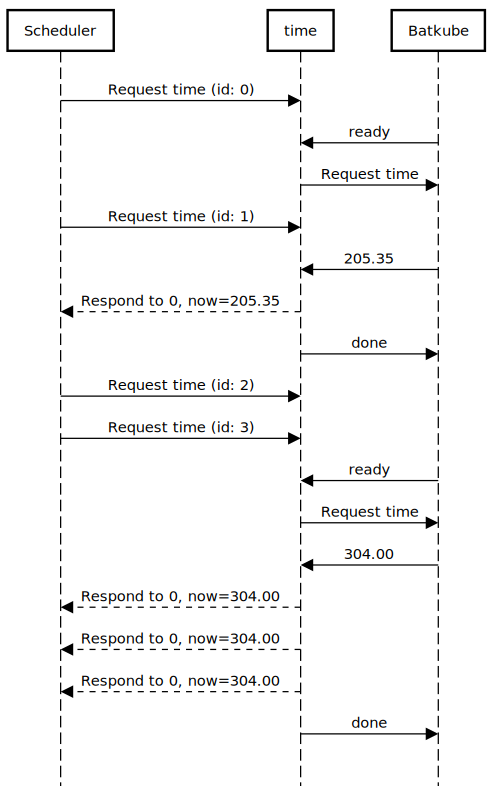
\includegraphics[scale=0.38]{../imgs/requester-broker.pdf}
		
		\column{0.5\textwidth}
		Exchanges between the scheduler, batsky-go (``time'') and Batsim
	\end{columns}
\end{frame}

\begin{frame}{Similar resources}
	\begin{columns}
		\column{0.5\textwidth}
		\centering
		\includegraphics[width=\textwidth]{../imgs/node-overview.png}
		\tiny{source: \url{https://kubernetes.io/docs/tutorials/kubernetes-basics/explore/explore-intro/}}

		\column{0.5\textwidth}
		\begin{block}{Translation between Kubernetes and Batsim}
			\begin{itemize}
				\item A Pod = a job.
				\item A Node = a compute resource.
			\end{itemize}
		\end{block}
	\end{columns}
\end{frame}

\begin{frame}{Realistic workload results}
	\centering
	\includegraphics[width=0.8\textwidth]{../imgs/timeout_realistic.png}
	\includegraphics[width=0.8\textwidth]{../imgs/max-timestep_realistic.png}
\end{frame}

\backupend
\end{document}
